\documentclass[11pt]{article}

%%
%% PACKAGES
%%

\usepackage[letterpaper, includeheadfoot, margin=0.9in,top=0.7in,bottom=0.8in]{geometry}
\usepackage[charter]{mathdesign} % Main font
\usepackage[scaled]{beramono} % Lovely monospace font
\usepackage[T1]{fontenc}
%\usepackage{amsmath, amssymb}
\usepackage{bm}
\usepackage{mathtools}
\usepackage{mathdots}
\usepackage{titlesec} % Custom section headings.
\usepackage{microtype}
\usepackage{xcolor}
\usepackage{xspace}
\usepackage{xfrac}
\usepackage{calc}
\usepackage{outlines}
\usepackage{natbib}

% Graphics.
%\usepackage{graphicx}
\usepackage{overpic}
\usepackage[update,prepend]{epstopdf} % To use eps files.

% Code listings.
\usepackage{listings} % Code listings.
\usepackage{matlab-prettifier} % MATLAB code listings

% Tweaks for captions and enumerations.
\usepackage[labelfont=bf]{caption} % Figure captions.
\usepackage{enumitem} % Fine tuning enumerations.
%\usepackage{floatrow} % Captions to the right of figures.

% Plotting and drawing
\usepackage{tikz} % This automatically loads graphicx!
\usetikzlibrary{calc} % For relative positions to defined coords
\usepackage{pgfplots} % Scientific plotting tools
\pgfplotsset{compat=1.7}

% Figure placement
%\usepackage{wrapfig}
%\captionsetup[wrapfigure]{margin=0.5cm}

% Packages to makes tables pretty.
\usepackage{array}
\usepackage{booktabs}
\setlength{\heavyrulewidth}{1.5pt}
\setlength{\abovetopsep}{4pt}
\renewcommand{\arraystretch}{1.2}

% Fancyhdr package stuff...
\usepackage{fancyhdr}
\setlength{\headheight}{30pt}
%\renewcommand{\headrulewidth}{0pt}
%\renewcommand{\footrulewidth}{0pt}

%%
%% SETTINGS
%%

% Path to look for graphics
\graphicspath{{../images/}}
%\epstopdfsetup{outdir=../images/}

% Caption spacing
\setlength{\abovecaptionskip}{0pt}

% List spacing
\setlist{noitemsep}

% Math operator font
\DeclareSymbolFont{sfoperators}{OT1}{cmss}{m}{n}
\DeclareSymbolFontAlphabet{\mathsf}{sfoperators}
\makeatletter
\def\operator@font{\mathgroup\symsfoperators}
\makeatother

%% No indent all paragraphs
%\setlength{\parindent}{0in}

% Figure references
\newcommand{\figref}[1]{Figure~\ref{#1}}

% Special format section headings
\titleformat{\section}%
	{\large\bf\scshape}% Text formatting
	{\arabic{section}}% Number
	{1em}% Space between number and text
	{}% Code before
	[]% Code after
\titleformat{\subsection}%
	{\normalsize\bf\scshape}% Text formatting
	{\arabic{section}.\arabic{subsection}}% Number
	{1em}% Space between number and text
	{}% Code before
	[]% Code after
%\titleformat{\subsubsection}%
%	{\color{blue}}% Text formatting
%	{\arabic{subsubsection} $\rightarrow$}% Number
%	{1em}% Space between number and text
%	{}% Code before
%	[]% Code after

%\definecolor{mygray}{rgb}{0.4, 0.4, 0.4}
%\lstset{
%style=Matlab-editor,
%mlscaleinline=false,
%basicstyle=\ttfamily\lst@ifdisplaystyle\scriptsize\fi,
%frame=single,
%rulecolor=\color{mygray},
%numbers=left,
%numbersep=10pt,
%numberstyle=\footnotesize \ttfamily \color{mygray},
%xleftmargin=30pt,
%xrightmargin=5pt,
%framexleftmargin=4pt,
%framextopmargin=2pt
%}
\lstset{
basicstyle=\ttfamily
}

% Allow white-space to be eaten within any lst environments between returns.
\lstset{breaklines,breakatwhitespace}

% Define a chacacter as shorthand for inline listings.
\lstMakeShortInline[basicstyle=\color{cyan!60!black}\small]{|}

%%
%% COMMANDS
%%

% Various plot lines to include in-line.
\newcommand{\solidrule}[1][8mm]{\rule[0.5ex]{#1}{1.5pt}}
\newcommand{\dashrule}{\mbox{%
	\solidrule[2mm]\hspace{1mm}\solidrule[2mm]\hspace{1mm}\solidrule[2mm]}}
\newcommand{\dotdashrule}{\mbox{%
	\solidrule[0.5mm]\hspace{1mm}\solidrule[2mm]\hspace{1mm}\solidrule[0.5mm]\hspace{1mm}\solidrule[2mm]}}

% Automated file inclusion for code listings
\makeatletter
\def\includecode{\@ifnextchar[{\@with}{\@without}}
\def\@with[#1]#2{
}
\def\@without#1{
  \lstinputlisting[caption=\ttfamily\protect\detokenize{#1}, escapechar=, frame=single]{../matlab_code/#1}
}
\makeatother

% Degree symbol.
\newcommand{\degree}{\ensuremath{^\circ}}

% Superscript text: 1st, 2nd, 3rd, 4th
\newcommand{\suptext}[1]{\ensuremath{^\text{#1}}\xspace}
\newcommand{\st}{\suptext{st}}
\newcommand{\nd}{\suptext{nd}}
\newcommand{\rd}{\suptext{rd}}
\let\oldth\th % Reassign the current \th command
\renewcommand{\th}{\suptext{th}}

% Underline matrices
\newcommand{\ul}[1]{\smash{\underline{#1}}}
\newcommand{\uul}[1]{\smash{\underline{\underline{#1}}}}

% Partial derivatives
\newcommand{\pp}[2]{\ensuremath{\frac{\partial#1}{\partial#2}}}

% Error function
\DeclareMathOperator\erf{erf}

% Big O notation
\newcommand{\bigo}{\ensuremath{\mathcal{O}}}

% Citation flag
\newcommand{\citeme}{{\color{red}\textbf{[cite]}}}

% Derivatives
\newcommand{\dd}[2]{\ensuremath{\frac{d #1}{d #2}}}
\newcommand{\pdd}[2]{\ensuremath{\frac{\partial #1}{\partial #2}}}
\newcommand{\tdd}[2]{\ensuremath{d #1 / d #2}}
\newcommand{\tpdd}[2]{\ensuremath{\partial #1 / \partial #2}}

% Text max and min
\newcommand{\tmax}{\ensuremath{\text{max}}}
\newcommand{\tmin}{\ensuremath{\text{min}}}

% Norm
\newcommand{\norm}[1]{\ensuremath{\left| #1 \right|}}

% Bold vectors
% Option 1: Works on more than single tokens, but makes regular letters italic as well as bold.
%\renewcommand{\vec}[1]{\mathbold{#1}}
% Option 2: Only works if a single token is passed to the command, but makes regular letters bold only.
\newcommand{\mb}[1]{
	\ifcat\noexpand#1\relax
		\expandafter\mathbold
	\else
		\expandafter\mathbf
	\fi{{#1}}
}

% Underlines for tensor notation.
\newcommand{\tsr}[1]{\ensuremath{\underline{#1}}}
\newcommand{\tsrr}[1]{\ensuremath{\underline{\underline{#1}}}}

% Allow lstinline within math mode. At bottom of this file b/c of syntax highlighting.
%\usepackage{letltxmacro}
%\newcommand*{\SavedLstInline}{}
%\LetLtxMacro\SavedLstInline\lstinline
%\DeclareRobustCommand*{\lstinline}{%
%  \ifmmode
%    \let\SavedBGroup\bgroup
%    \def\bgroup{%
%      \let\bgroup\SavedBGroup
%      \hbox\bgroup
%    }%
%  \fi
%  \SavedLstInline
%}


%%
%% DOCUMENT START
%%

\begin{document}
\fancypagestyle{allpages}
{
	\fancyhf[LH]{\rightmark}
	\fancyhf[CH]{}
	\fancyhf[RH]{\thepage\hspace*{1ex}/\hspace*{1ex}\pageref{lastpage}}
	\fancyhf[LF]{}
	\fancyhf[CF]{}
	\fancyhf[RF]{}
}

\fancypagestyle{firstpage}
{
	\fancyhf[LH]{\Large Final Project \\ \large ASEN 6519: Uncertainty Quantification}
	\fancyhf[CH]{}
	\fancyhf[RH]{\large Ryan Skinner \\ \large Due 2016/??/??}
	\fancyhf[LF]{}
	\fancyhf[CF]{}
	\fancyhf[RF]{}
}

\pagestyle{allpages}
\thispagestyle{firstpage}
\renewcommand{\sectionmark}[1]{ \markright{#1}{} }

\vspace*{0in}
\begin{center}
\LARGE Impact of Geometric Uncertainty on a NACA 4412 Airfoil
\end{center}
\vspace*{0.3in}

%%%%%%%%%%%%%%%%%%%%%%%%%%%%%%%%%%%%%%%%%
%%%%%%%%%%%%%%%%%%%%%%%%%%%%%%%%%%%%%%%%%
\section{Introduction}
%%%%%%%%%%%%%%%%%%%%%%%%%%%%%%%%%%%%%%%%%
%%%%%%%%%%%%%%%%%%%%%%%%%%%%%%%%%%%%%%%%%

%%%%%%%%%%%%%%%%%%%%%%%%%%%%%%%%%%%%%%%%%
%%%%%%%%%%%%%%%%%%%%%%%%%%%%%%%%%%%%%%%%%
\section{Problem Definition}
%%%%%%%%%%%%%%%%%%%%%%%%%%%%%%%%%%%%%%%%%
%%%%%%%%%%%%%%%%%%%%%%%%%%%%%%%%%%%%%%%%%

%%%%%%%%%%%%%%%%%%%%%%%%%%%%%%%%%%%%%%%%%
%%%%%%%%%%%%%%%%%%%%%%%%%%%%%%%%%%%%%%%%%
\section{Implementation}
%%%%%%%%%%%%%%%%%%%%%%%%%%%%%%%%%%%%%%%%%
%%%%%%%%%%%%%%%%%%%%%%%%%%%%%%%%%%%%%%%%%

The shape of a 4-digit NACA xyzz airfoil is specified by three geometric parameters, all non-dimensionalized with respect to the chord length $c$:
\begin{itemize}
\item $m = \text{x} / 100$ is the maximum camber
\item $p = \text{y} / 10$ is the location of maximum camber
\item $t = \text{zz}/100$ is the maximum thickness
\end{itemize}

For a physical coordinate $x \in [0, c]$, the thickness of a symmetric airfoil is given by
\begin{equation}
y_t = 5tc\, \left[ 0.2969 \sqrt{\frac{x}{c}} + (-0.1260) \left(\frac{x}{c}\right) + (-0.3516) \left(\frac{x}{c}\right)^2 + 0.2843 \left(\frac{x}{c}\right)^3 + (-0.1015) \left( \frac{x}{c} \right)^4 \right]
\end{equation}
The coordinate pairs of points on the upper $(x_U, y_U)$ and lower $(x_L, y_L)$ surface are simply $x_U = x_L = x$, $y_U = y_t$, and $y_L = -y_t$. A symmetric airfoil corresponds to the NACA 00zz series. One example is NACA 0012, shown in \figref{fig:naca0012}.

Cambered NACA airfoils define thickness perpendicular to the camber line, which can be defined as
\begin{equation}
y_c = \begin{cases}
m \frac{x}{p^2} \left( 2p-\frac{x}{c}\right) & 0 \le x \le pc \\
m \frac{c-x}{(1-p)^2} \left(1-2p+\frac{x}{c}\right) & pc \le x \le c
\end{cases}
\end{equation}
The upper and lower coordinate pairs become
\begin{equation}
\begin{aligned}
x_U &= x - y_t \sin \theta &\quad y_U &= y_c + y_t \cos \theta \\
x_L &= x + y_t \sin \theta &\quad y_L &= y_c - y_t \cos \theta
\end{aligned}
\end{equation}
where
\begin{equation}
\theta = \arctan \left( \dd{y_c}{x} \right)
\quad \text{and} \quad
\dd{y_c}{x} =
\begin{cases}
\frac{2m}{p^2} \left( p - \frac{x}{c} \right) & 0 \le x \le pc \\
\frac{2m}{(1-p)^2} \left( p - \frac{x}{c} \right) & pc \le x \le c
\end{cases}
\end{equation}

Because cambered profiles are generated from their symmetric counterparts, we can analytically determine the displacements necessary to deform any symmetric NACA mesh into an arbitrary 4-digit NACA mesh. This results in substantial efficiency gains. In our case, we create a CAD model of a NACA 0012 airfoil, mesh it, and partition it once. Then, in the initialization stage of a new simulation, we generate a stochastic NACA realization parameterized by random variables $\mb{m}$, $\mb{p}$, and $\mb{t}$. Each mesh node on the airfoil surface is prescribed a displacement based on its $x$-coordinate, which is then passed to a linear elastic structural solver. Numerical solution of the unsteady incompressible Navier-Stokes equations proceeds on the deformed mesh.

\begin{figure}[b]
\begin{center}
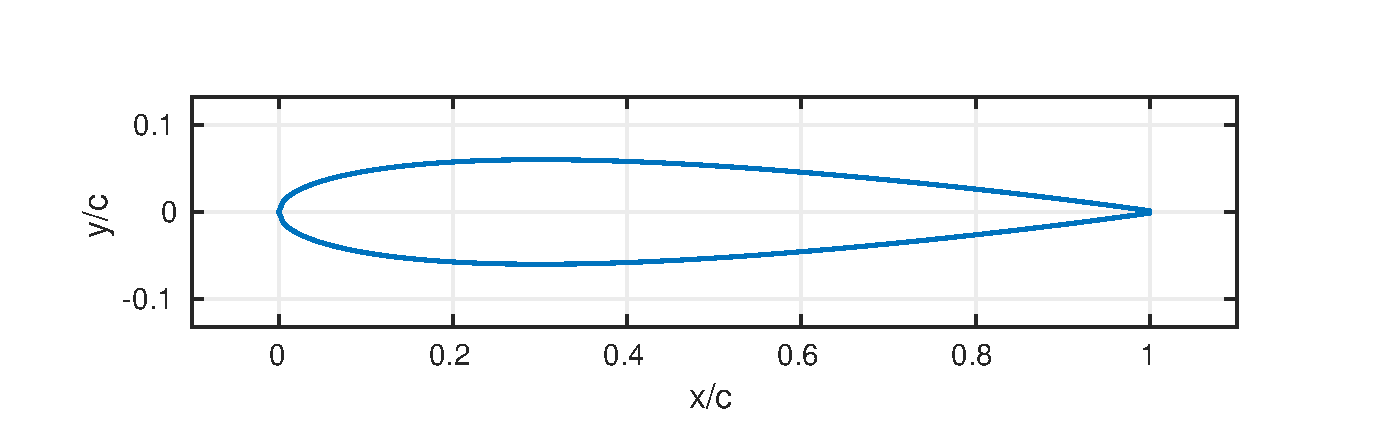
\includegraphics[width=0.85\textwidth]{naca0012.eps}
\vspace{1ex}
\caption{Surface of a NACA 0012 airfoil.}
\label{fig:naca0012}
\end{center}
\end{figure}




%%
%% DOCUMENT END
%%
\label{lastpage}
\end{document}



























